\documentclass{beamer}
%\usetheme{Boadilla}
\usetheme{default}

\usepackage{epstopdf}
\usepackage{listings}
\usepackage{subcaption}
\usepackage[utf8]{inputenc}
%\usepackage{unicode-math}
\usepackage{alltt}
\usepackage{booktabs}
\usepackage{fancyvrb}
\usepackage{multicol}

% In descriptions, start new line after label
\usepackage{enumitem}
\setlist[description]{style=nextline}

\newcommand{\tuple}[1]{\langle #1 \rangle}

\usepackage{fontspec}
%\setmonofont[Scale=0.85]{DroidSansMono.ttf}
\setmonofont[Scale=0.95]{inconsolata}

\title{Arrp}
\subtitle{A Programming Language for Signal Processing}
\author{Jakob Leben}
\institute{Limbic Media, Victoria, Canada}
\date{Lyon, December 14, 2019}

\begin{document}

\begin{frame}
\titlepage
\end{frame}

\begin{frame}
\frametitle{Outline}
\tableofcontents
\end{frame}

\section{Motivation}

\begin{frame}[t, fragile]
\frametitle{Stream Programming Landscape}

\begin{center}
← larger scale / smaller scale →


\includegraphics{../figures/landscape_before_arrp}
\end{center}
\begin{minipage}[t]{0.48\linewidth}
\begin{center}
Streaming languages\\
+ convenient\\
− restricted

\vspace{10pt}

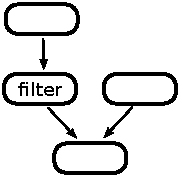
\includegraphics{../figures/stream-graph}
\end{center}
\end{minipage}\hfill
\begin{minipage}[t]{0.48\linewidth}
\begin{center}
General-purpose languages\\
− inconvenient\\
+ powerful

\vspace{10pt}

\small
\begin{BVerbatim}
class filter
{
  filter(params...)
  {...}

  void process
  (const float * in, float * out)
  {...}
}
\end{BVerbatim}
\end{center}
\end{minipage}
\end{frame}

\begin{frame}[t, fragile]
\frametitle{Stream Programming Landscape}

\begin{center}
← larger scale / smaller scale →

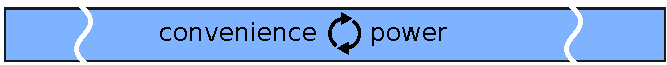
\includegraphics{../figures/landscape_after_arrp}
\end{center}
\begin{center}
Arrp\\
+ fairly convenient\\
+ fairly powerful
\end{center}
\begin{minipage}[t]{0.48\linewidth}
\begin{center}
Streaming languages\\
+ convenient\\
− restricted
\end{center}
\end{minipage}\hfill
\begin{minipage}[t]{0.48\linewidth}
\begin{center}
General-purpose languages\\
− inconvenient\\
+ powerful
\end{center}
\end{minipage}

\end{frame}

\begin{frame}[fragile]
\frametitle{Performance with High-Volume Streams}
\includegraphics[width=\textwidth]{../build/parallel-scaling-slide}
\end{frame}

\section{Features}

\begin{frame}[fragile]
\frametitle{Familiar syntax}

\textbf{One-pole filter}
\[y[n] = b\,x[n] - a\,y[n-1]\]
\begin{center}
\begin{BVerbatim}
y[n] = b*x[n] - a*y[n-1];
\end{BVerbatim}
\end{center}

\textbf{FIR filter}
\[y[n] = \sum_{i = 0}^{N-1} \; b[i]\,x[n-i]\]
\begin{center}
\begin{BVerbatim}
y[n] = sum([i:N] -> b[i] * x[n-i])
\end{BVerbatim}
\end{center}

\textbf{Max filter}
\[y[n] = \max_{i = 0}^{N-1} \; x[n+i]\]
\begin{center}
\begin{BVerbatim}
y[n] = max_elem([i:N] -> x[n+i]);
\end{BVerbatim}
\end{center}

\end{frame}


\begin{frame}[fragile]
\frametitle{Polymorphic, higher-order functions}

\begin{center}
\begin{BVerbatim}
max_filter(N,x) = y where
    y[n] = max_elem([i:N] -> x[n+i]);

max_elem = fold((a,b) -> max(a,b));

fold(f,x) = r[#x-1] where {
    r[0] = x[0];
    r[i] = f(r[i-1], x[i]), if i < #x;
}
\end{BVerbatim}
\end{center}

\end{frame}



\begin{frame}[fragile]
\frametitle{Point-wise Operations, Multi-dimensional Streams}

\begin{center}
\begin{BVerbatim}
max_filter(N,x) = y where
    y[n] = max_elem([i:N] -> x[n+i]);

input x1 : [~]real32;
y1 = max_filter(10, x1);

input x2 : [~,10]real32;
y2 = max_filter(15, x2);
\end{BVerbatim}
\end{center}

\end{frame}


\begin{frame}[fragile]
\frametitle{Multi-rate Programs}

\begin{center}
\begin{BVerbatim}
downsample(x, factor) = [n] -> x[factor * n];

upsample(x, factor) = y where
    y[n] = {
        x[n / factor], if n % factor == 0;
        0,             otherwise
    };

max_filter(N, hop, x) = y where
    y[n] = max_elem([i:N] -> x[hop * n + i]);
\end{BVerbatim}
\end{center}

\end{frame}


\begin{frame}[fragile]
\frametitle{Physical Modeling}

\textbf{2d Wave Equation - FDTD\footnotemark}
\begin{center}
\begin{BVerbatim}
u[n,i,j] =
      b0 * u[n-2, i, j]
    + b1 * u[n-1, i, j]
    + b2 * (  u[n-1, i+1, j] + u[n-1, i, j+1]
            + u[n-1, i-1, j] + u[n-1, i, j-1] );
\end{BVerbatim}
\end{center}

\footnotetext{Stefan Bilbao. Numerical Sound Synthesis:
Finite Difference Schemes and Simulation in Musical Acoustics. 2009.}
\end{frame}

\section{Example of Usage}

\begin{frame}[fragile]
\frametitle{Example: One-Pole Filter}

\centering

\begin{BVerbatim}
input a : real64;
input b : real64;
input x : [~]real64;
output y : [~]real64;

y[0] = 0;
y[n] = b*x[n] - a*y[n-1];
\end{BVerbatim}

\end{frame}


\begin{frame}[fragile]
\frametitle{Generated C++}

\footnotesize
\begin{minipage}{0.49\linewidth}
\begin{BVerbatim}
template <typename IO>
class program
{
public:
  IO * io;
  void prelude();
  void period();
private:
  double a;
  double y;
  double b;
};
\end{BVerbatim}
\end{minipage}\hfill
\begin{minipage}{0.49\linewidth}
\begin{BVerbatim}
template <typename IO>
inline void program<IO>::prelude()
{
  double x;
  io->input_b(b);
  io->input_a(a);
  y=0;
  io->input_x(x);
  io->output_y(y);
}

template <typename IO>
inline void program<IO>::period()
{
  double x;
  io->input_x(x);
  y=b*x-a*y;
  io->output_y(y);
}
\end{BVerbatim}
\end{minipage}

\end{frame}


\begin{frame}[fragile]
\frametitle{Generated Executable}

\small

\begin{Verbatim}
ffmpeg -i input.wav -ac 1 -ar 44.1k -f f64le pipe:1 |
\end{Verbatim}

{
\bf
\begin{Verbatim}
./filter --format=raw a=0.5 b=0.5 |
\end{Verbatim}
}

\begin{Verbatim}
ffmpeg -y -ac 1 -ar 44.1k -f f64le -i pipe:0 file:output.wav
\end{Verbatim}

\end{frame}

\section{Future Work}

\begin{frame}[fragile]
\frametitle{Future Work}

\begin{itemize}
\item Standard library
\item Integration with other systems (SuperCollider, Max/MSP, LV2, Bela, ...)
\item Parametric array sizes
\item Support for implementation of algorithms like FFT
\item Automatic optimization
\end{itemize}

\end{frame}

\begin{frame}[fragile]

\centering

Thank you.

\vspace{15pt}

Arrp Website: http://arrp-lang.info

\vspace{30pt}

Jakob Leben, Victoria, Canada

jakob.leben@gmail.com

\end{frame}

\end{document}

